\chapter{Cifratura Simmetrica - DES}
In crittografia un algoritmo di cifratura a blocchi è un algoritmo a chiave simmetrica che opera su un gruppo di bit di lunghezza 
finita organizzati in un blocco. I blocchi vengono cifrati contemporaneamente.

\noindent Con blocchi da $n$ bit in chiaro, si ottengono $2^n$ possibili input; quando avviene la trasformazione da blocco in chiaro a blocco cifrato,
occore che essa sia univoca e \textbf{reversibile}; significa che ogni blocco in chiaro deve produrre un blocco cifrato univoco.

\noindent La chiave è ciò che effettua questa mappatura tra blocchi in chiaro e blocchi cifrati; se ho un blocco di $n$ bit, la chiave deve 
avere una lunghezza di almeno $n \cdot 2^n$ affinché possa coprire tutte le possibili mappature. 

\noindent L'idea è che ogni valore del blocco 
venga mappato su un altro valore del blocco (quindi con una mappatura 1:1). Ad esempio, con un blocco di due bit:

\begin{figure}[H]
    \centering
    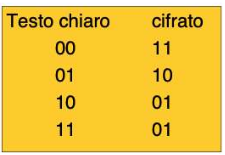
\includegraphics[width=0.3\linewidth]{chapters/chap4/images/mappatura.png}
\end{figure}

\noindent I blocchi piccoli equivalgono ad una cifratura a sostituzione (vulnerabili dunque ad analisi statistica), mentre i blocchi di grandi 
dimensioni portano a problemi relativi alla dimensione della chiave.

\noindent Le operazioni di \textbf{cifratura e decifratura} vengono svolte consultando la tabella di mappatura.

\section{Cifratura di Feistel}

Un cifrario di Feistel è un \textbf{algoritmo di cifratura a blocchi} con una particolare struttura, usata da molti algoritmi. Ha il vantaggio 
che \textbf{la cifratura e decifratura sono molto simili}, spesso identiche, e che basta invertire il funzionamento del gestore della chiave 
per ottenere l'operazione inversa (permettendo di usare gli stessi circuiti).

\noindent L'idea è quella di usare \textbf{cifrature in sequenza} per ottenere cifrature più complesse di una singola componente, alternando 
operazioni di sostituzione e permutazione; queste operazioni, reiterate più volte (\textit{round}), conferiscono all'algoritmo le proprietà di \textbf{confusione}
e \textbf{diffusione}:
\begin{itemize}
    \item \textbf{confusione:} consiste nel rendere la correlazione tra la chiave e il testo cifrato il meno correlata possibile; cerca di non permettere 
    di risalire alla chiave dal cifrato 
    \item \textbf{diffusione:} è la capacità dell'algoritmo di distribuire le correlazioni statistiche del testo lungo tutto l'alfabeto 
    usato, rendendo quanto più difficile un attacco statistico
\end{itemize}

\noindent Queste sono due proprietà che un agoritmo di cifratura \textbf{deve possedere affinché sia considerabile robusto}, ovvero scarsamente 
attaccabile attraverso la crittoanalisi perché in grado di contrastare attacchi statistici.

\subsubsection{Caratteristiche}
Le caratteristiche dei cifrari di Feistel sono le seguenti:
\begin{itemize}
    \item \textbf{Dimensione del blocco:} maggiore è la dimensione, maggiore sarà la sicurezza (al prezzo di prestazioni peggiori)
    \item \textbf{Dimensione della chiave:} analogo alle considerazioni sulla dimensione del blocco 
    \item \textbf{Numero di fasi:} tutte le fasi hanno la stessa struttura 
    \item \textbf{Algoritmo di schedulazione della chiave:} a partire dalla chiave iniziale, vengono prodotte tante sottochiavi quanti sono i round
    \item \textbf{Funzione da usare ogni round:} maggiore è la complessità, maggiore sarà la resistenza alla crittoanalisi 
\end{itemize}

\noindent Poniamo $F$ la funzione dei passaggi e $K_0, K_1, \dots, K_n$ le sottochiavi dei passaggi $0, 1, \dots , n$. Il procedimento è:
\begin{itemize}
    \item l'input viene diviso in due parti uguali $L_0$ e $R_0$
    \item per ogni round $i$ viene calcolato 
    \begin{center}
        $L_i = R_{i-1}$ e $R_i = L_{i-1} \bigoplus f(R_{i-1}, K_{i-1})$
    \end{center}

    \noindent con $f$ funzione di round e $K_i$ chiave di sessione
\end{itemize}

$\Rightarrow$ così facendo si ottiene il testo cifrato $(L_n, R_n)$

\newpage
\noindent Senza considerare la funzione $f$, la decifrazione si ottiene con 

\begin{center}
    $R_{i-1} = L_i$ e $L_{i-1} = R_i \bigoplus f(L_i, K_i)$
\end{center}

\noindent $\rightarrow$ il procedimento è invertibile indipendentemente da $f$, permettendo di scegliere funzioni $f$ non invertibili 
e molto complesse.

\begin{figure}[H]
    \centering
    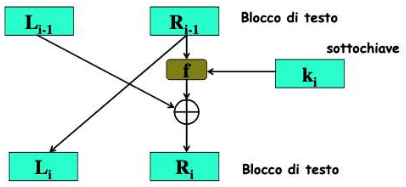
\includegraphics[width=0.7\linewidth]{chapters/chap4/images/feistel.png}
\end{figure}



\section{DES}

È un algoritmo di cifratura a blocchi che usa:
\begin{itemize}
    \item dimensione del blocco di 64 bit 
    \item chiave di 64 bit, di cui 56 bit usati effettivamente dall'algoritmo e 8 usati per il controllo di parità (per ciascun byte, 
    i primi 7 bit sono parte della chiave mentre l'ultimo è usato per il controllo (corrisponde allo XOR dei precedenti 7))
\end{itemize}

\begin{figure}[H]
    \centering
    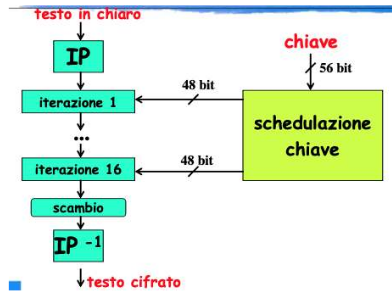
\includegraphics[width=0.7\linewidth]{chapters/chap4/images/des.png}
\end{figure}

\noindent Come schematizzato nell'immagine, ci sono 16 fasi identiche dette \textit{round}, necessarie per ottenere una diffusione sufficiente. Ci sono poi due 
operazioni di permutazione, $IP$ all'inzio e $IP^{-1}$ alla fine, che si annullano (sono dunque inutili ai fini di cifratura) probabilmente 
usate per facilitare il caricamento dei blocchi sull'hardware degli anni '70.

\noindent Prima del ciclo principale, il \textbf{blocco viene suddiviso in due metà} e processao alterativamente; questo incrocio viene detto 
\textit{rete di Feistel}. La struttura della rete assicura che cifratura e decifratura siano processi simili.  La funzione (che è quella vista 
in precedenza) non fa altro che mescolare una metà del blocco con una parte della chiave; il risultato viene poi combinato con l'altra metà 
del blocco e le due metà vengono scambiate prima del ciclo successivo.

\noindent La singola funzione $f$ (vista in precedenza) opera su 4 passi:
\begin{itemize}
    \item \textbf{Espansione:} il mezzo blocco di 32 bit viene espanso fino a 48 bit usando una permtuazione di espansione (E nel blocco che segue)
    \item \textbf{Miscelazione con la chiave:} il risultato è combinato con una sottochiave usando un'operazione di XOR; 16 sottochiavi di 48 bit, una 
    per ogni ciclo, sono derivate dalla chiave principale usando il gestore della chiave 
    \item \textbf{Sostituzione:} il blocco viene diviso in 8 parti da 6 bit ciascuna che vengono processati con la \textit{substitution box} (s-box); ognuna delle 8 parti 
    sostituisce 6 bit in input con 4 in output mediante uan trasformazione non lineare; le s-box forniscono il \textbf{principale elemento di sicurezza di DES}, siccome 
    senza di esse la cifratura sarebbe lineare
    \item \textbf{Permutazione:} i 32 bit risultanti dalle s-box sono riordinati in base alle permutazioni fisse (p-box)
\end{itemize}

$\rightarrow$ l'alternanza di s-box e p-box garantiscono sia diffusione che confusione 

\noindent Il \textbf{gestore delle chiavi di cifratura}, ovvero quello che genera le sottochiavi a partire dalla chiave iniziale, funziona 
secondo i seguenti passi:
\begin{itemize}
    \item vengono selezionati 56 dei 64 bit iniziali tramite una funzione detta \textbf{permuted choice 1}; i restanti 8 sono scartati e usati 
    come controllo di parità; nella funzione \textit{PC1}, i bit di parità sono multipli di 8 
    \item i 56 bit sono divisi in due parti di 28 bit che verranno trattate separatamente; nei cicli vengono fatte un totale di 28 permutazioni 
    \item a questo punto vengono scelti, per ogni round, 24 bit da ciascuno dei due sottoinsiemi ottenuti mediante la funzione \textbf{permuted choice 2}
\end{itemize}

\subsection{Modalità operative}

In crittografia la \textit{modalità operativa} di un cifrario a blocchi è una serie di procedimenti standard per garantire la sicurezza; le modalità 
operative di DES sono:
\begin{itemize}
    \item \textbf{Electronic Codebook Chaining (ECB):} è la più semplice; il testo in chiaro viene suddiviso in blocchi da 64 bit; a parità di testo 
    e di chiave, il cifrato sarà sempre lo stesso; non è adatto a messaggi lunghi 
    \item \textbf{Cipher Block Chaining (CBC):} supera il limite di ECB (a parità di testo e di chiave, si ottiene un cifrato differente). L'input è dato 
    dallo XOR tra il blocco di testo corrente e il blocco cifrato precedente (per ciascun blocco viene usata la stessa chiave).

    \noindent Il primo blocco viene cifrato con un  \textit{inizialization vector}, che deve essere noto anche al destinatario per permette la decifratura; per evitare attacchi 
    di \textit{replay}, l'$iv$ viene modificato per ogni istanza di esecuzione.

    \noindent La dipendenza tra i blocchi genera un \textbf{rallentamento} e rende l'algoritmo soggetto alla \textbf{propagazione degli errori}.

    \item \textbf{Cipher Feedback (CFB):} idealmente si vuole \textbf{convertire una cifratura a blocchi in una a flusso}; il processo di cifratura 
    avviene utilizzando un registro di scorrimento a 64 bit che, inizialmente, contiene l'$iv$. I primi $s$ bit del testo in chiaro vengono posti a XOR 
    con i primi $s$ bit dell'$iv$; a questo punto, si fa scorrere di $s$ bit il contenuto del registro e gli ultimi $s$ bit, che rimmarrebbero vuoti, sono 
    riempiti con i bit cifrati appena calcolati.

    \noindent Il valore di $s$ può essere scelto a piacimento. Questo approccio ha lo svantaggio di essere soggetto alla \textbf{propagazione degli errori}
    e di non essere efficiente per valori di $s$ piccoli
    
    \item \textbf{Counter (CTR):} viene usato un contatore; il requisito fondamentale è che sia diverso per ogni blocco. Per la cifratura, viene fatto lo
    XOR tra il contatore (cifrato) e il testo in chiaro; per la decifratura si usa la stessa sequenza di valori del contatore con il testo cifrato. Ha i vantaggi di:
    \begin{itemize}
        \item \textit{efficienza hw e sw;} l'esecuzione può essere fatta in parallelo su più blocchi
        \item \textit{pre-elaborazione;} è possibile precalcolare l'output 
        \item \textit{accesso casuale}
        \item \textit{sicurezza dimostrabile}
        \item \textit{semplice}, siccome richiede solo l'algoritmo crittografico 
    \end{itemize}
\end{itemize}

\section{Sicurezza dei cifrari moderni}
Con \textbf{sicurezza perfetta} intendiamo che un attaccante non possa ricavare alcuna informazione del testo cifrato. 

\noindent Con \textbf{sicurezza computazionale} intendiamo che se dotato di abbastanza tempo e risorse, un attaccante possa rompere il cifrario (è quindi 
un rilassamento della sicurezza perfetta). 

\noindent La sicurezza perfetta prevede quindi che l'avversario sia dotato di capacità computazionali e temporali illimitate, ma che non riesca 
comunque a ottenere alcuna informazione dal testo cifrato. Nella pratica, uno schema che rivela informazioni con probabilità $2^-60$ ad avversari 
che possono investire 200 anni di sforzo computazionale è considerato molto buono. 

Esistono due approcci che mirano a garantire la sicurezza di un cifrario:
\begin{itemize}
    \item concreto 
    \item asintotico
\end{itemize}

\subsection{Approccio concreto}

Limita la probabilità di successo massima di qualsiasi avversario che esegua un attacco per una specifica quantità di tempo.

\noindent Uno schema $(t, \epsilon)$ è sicuro se qualsiasi avversario che ha a disposizione tempo $t$ riesce a rompere lo schema con 
probabilità $\epsilon$.

\noindent I cifrari moderni sono considerati ottimali se, con una chiave di lunghezza $n$, un avversario riesce a rompere lo schema con probabilità $1/2^n$ adottando un 
attacco di forza bruta.

\subsection{Approccio asintotico}
Nell'ambito della sicurezza computazionale, uno schema è considerato sicuro se un avversario che opera in tempo polinomiale rompe lo schema 
con probabilità trascurabile. Introduce un parametro di sicurezza $n$ intero, utilizzato per parametrizzare sia lo schema che lo parti coinvolte;
è noto agli avversari, e i tempi di esecuzione degli avversari e la probabilità di successo sono espresse in funzione di $n$:

\noindent Il parametro $n$ permette di calibrare la sicurezza dello schema di cifratura al livello desiderato, considerando $n$ come la 
lunghezza della chiave; il tempo di ricerca della chiave deve crescere in maniera esponenziale rispetto alla lunghezza delle chiave.

\section{Crittoanalisi di DES}
Il metodo più efficaciente per violare DES è un attacco di forza bruta (avendo una chiave di 56 bit). Esistono però altre due strategie:
\begin{itemize}
    \item crittoanalisi differenziale
    \item crittoanalisi lineare
\end{itemize}

\noindent Sono delle tecniche generali di crittoanalisi che hanno successo con molti cifrari.

\subsection{Forza bruta}
Un attacco di forza bruta è il metodo di attacco più semplice, in quanto consiste nel provare tutte le possibili chiavi; in DES, avendo una chiave 
a 56 bit, ci sono $2^56$ possibili chiavi. Nel caso di \textit{known plain text attack}, in genere bastano $2^55$ tentativi.

\noindent L'approccio a questo tipo di problema è legato al compromesso tra memoria e tempo di calcolo: si può efficientarne uno aumentando 
il costo dell'altro. È possibile creare una tabella di ricerca che tracci le corrispondenze tra testo in chiaro e cifrato per ogni chiave possibile; 
si può calcolare l'intera tabella (aumentando i costi di memoria) o solo alcune voci (aumentando il tempo di calcolo).

\noindent Nel momento in cui si ottiene il cifrato, la decifrazione si limiterà alla sola ricerca della chiave nella tabella; questo processo, che ha 
tempo di esecuzione costante o al più logaritmico, e spazio di memoria pari a $2^56$. L'idea per costruire
la tabella è quella di usare una funzione di riduzione che, data una stringa da 64 bit, ne ricava una di 56 bit. 

\noindent $\rightarrow$ data una stringa di 64 bit $x$, posso applicare la funzione di riduzione e usare quei 56 bit come chiave. Definiamo quindi 
$y = DES_{1,0}(x)$; riapplicando DES a $y$ con la stessa chiave otteniamo $x_{1,1}$.

\noindent Iterando questo processo arriviamo ad ottenere $x_{1,t}$, dove $t$ è il numero di colonne della tabella di ricerca. È possibile partire 
da chiavi diverse da quella precedenza, ottenendo così una tabella di $m$ righe (una per ogni chiave) e $t$ colonne.

\noindent Bisogna ricordare che il valore della chiave \textbf{potrebbe non essere esattamente quello} dato che il valore ottenuto è stato preso buttando 
8 bit dai 64 presi in partenza.


\textbf{fanculo è da finire sta parte}








